\documentclass[]{scrartcl}
\usepackage{lmodern}
\usepackage{amssymb,amsmath}
\usepackage{ifxetex,ifluatex}
\usepackage{fixltx2e} % provides \textsubscript
\ifnum 0\ifxetex 1\fi\ifluatex 1\fi=0 % if pdftex
  \usepackage[T1]{fontenc}
  \usepackage[utf8]{inputenc}
\else % if luatex or xelatex
  \ifxetex
    \usepackage{mathspec}
  \else
    \usepackage{fontspec}
  \fi
  \defaultfontfeatures{Ligatures=TeX,Scale=MatchLowercase}
\fi
% use upquote if available, for straight quotes in verbatim environments
\IfFileExists{upquote.sty}{\usepackage{upquote}}{}
% use microtype if available
\IfFileExists{microtype.sty}{%
\usepackage{microtype}
\UseMicrotypeSet[protrusion]{basicmath} % disable protrusion for tt fonts
}{}
\usepackage{hyperref}
\hypersetup{unicode=true,
            pdftitle={Angabe},
            pdfauthor={Team\ldots{}},
            pdfborder={0 0 0},
            breaklinks=true}
\urlstyle{same}  % don't use monospace font for urls
\IfFileExists{parskip.sty}{%
\usepackage{parskip}
}{% else
\setlength{\parindent}{0pt}
\setlength{\parskip}{6pt plus 2pt minus 1pt}
}
\setlength{\emergencystretch}{3em}  % prevent overfull lines
\providecommand{\tightlist}{%
  \setlength{\itemsep}{0pt}\setlength{\parskip}{0pt}}
\setcounter{secnumdepth}{5}
% Redefines (sub)paragraphs to behave more like sections
\ifx\paragraph\undefined\else
\let\oldparagraph\paragraph
\renewcommand{\paragraph}[1]{\oldparagraph{#1}\mbox{}}
\fi
\ifx\subparagraph\undefined\else
\let\oldsubparagraph\subparagraph
\renewcommand{\subparagraph}[1]{\oldsubparagraph{#1}\mbox{}}
\fi

\usepackage{graphicx}
\usepackage{array}
\usepackage{ragged2e}
\usepackage[section]{placeins}
\makeatletter
\AtBeginDocument{%
  \expandafter\renewcommand\expandafter\subsection\expandafter{%
    \expandafter\@fb@secFB\subsection
  }%
}
\makeatother
 
\title{Angabe 1}
\providecommand{\subtitle}[1]{}
\subtitle{Untertitel}
\author{Daniel Graf, Dimitrie Diez, Arne Schöntag, Peter Müller}
\date{}

\begin{document}
\maketitle


\tableofcontents

\section{Einführung}

% Problem -> Motivation

\section{Messexperiment}

Das Messexperiment wurde am $05.04.2017$ im Lichthof der Hochschule München (Lothstraße 64) durchgeführt. Es nahmen $22$ Probanden im Alter von $20-29$ Jahren teil. Das Experiment bestand aus drei Teilen. 

Zunächst wurde die Wunschgeschwindigkeit in der Ebene gemessen. Hierfür ging jeder Proband eine markierte Strecke von $27,3m$ ab und stoppte die hierfür benötigte Zeit. Anschließend wurde dieser Vorgang zweimal wiederholt und die entsprechende Rundennummer vermerkt. Im zweiten Teil erfolgte die Messung der benötigten Zeit für einen Treppenaufstieg. Die Treppenlänge betrug $9m$. Jeder Proband führte den Vorgang dreimal durch und vermerkte die benötigte Zeit und die entsprechende Rundennummer. Analog hierzu wurde im dritten Teil des Experiments die Zeit beim Treppenabstieg gemessen. 

Neben den gemessenen Zeiten in jeder Runde, dem Alter und der Körpergröße ist auch das Geschlecht jedes Probanden bekannt. Weitere Informationen sind in der beiliegenden Versuchsbeschreibung "Choreographie\_Treppengeschwindigkeit\_2017" aufgeführt. In den folgenden Kapiteln erfolgt die Auswertung der ermittelten Messwerte.

\section{Überprüfung auf Normalverteilung}
\section{Modell}
\section{Lineare Regression}
\subsection{Prüfung auf eine Abhängigkeit}
\subsection{Mehrere Abhängigkeiten}
\subsection{Konditionierung}

\section{Ergebnisse}
\section{Ermitteltes Modell}

\section{Vergleich mit Daten aus 2012}
\subsection{Überprüfung auf Normalverteilung}
\subsection{Lineare Regression}
\subsection{Vergleich}

\section{Verbund von alten und neuen Daten}
Unter der Annahme, dass die Bedingungen zum Zeitpunkt des Messeperimentes im Jahr 2012 ähnlich waren wie im Jahr 2017, kann man die erfassten Daten aus beiden Experimenten zu einem gemeinsamen Datensatz zusammenfassen. Dies kann von Vorteil sein, da es sich insgesamt um mehr Teilnehmer handelt, und so eine Aussagekraft der Berechnungen erhöht wird. Es ist jedoch zu bedenken, dass folgende Faktoren die Aussagekraft verringern können. Zum einen hat eine Abweichung der Messbedingungen von 2012 zum Jahr 2017 direkten Einfluss auf die Messergebnisse. Zum Beispiel hat die Treppenhöhe einen enormen Einfluss auf die Treppengeschwindigkeit. Darüber hinaus ist zu bemerken, dass unter Umständen in beiden Experimenten ein und die selbe Person teilgenommen hat und unter unterschiedlicher Probanden ID geführt wird. Dies kann zum Berispiel bedeuten, dass in den Datensätzen zwei Personen mit der gleichen Körpergröße gibt. Diese Doppelerfassung einer Person hat zur Folge, dass die betreffende Person die Auswertung mit mehr Gewicht beeinflußt. 
Für die weitere Auswertung wird angenommen, dass die Messbedingungen beider Experimente annähernd gleich sind und durch die lange Zeit zwischen den beiden Experimenten, es keine Doppelerfassungen von Personen gibt. Der Fokus liegt vor allem auf der Analyse der linearen Regression.
\subsection{Prüfung auf eine einfache Abhängigkeit}
\begin{figure}[htpb]
\centering
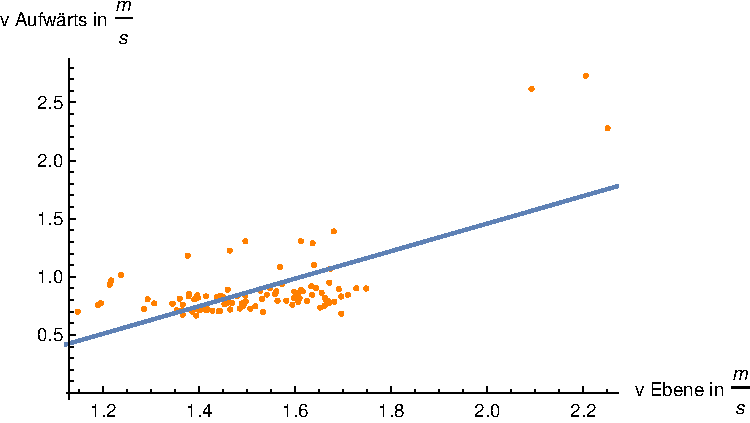
\includegraphics[width=0.7\textwidth]{abbildungen/regression/2012_2017_verbund/auf-ebene.pdf}
\label{fig:2012_und_2017_OA_auf_ebene}
\caption{aaaaa}
\end{figure}
\section{Fazit}

\end{document}